% Содержимое отчета по курсу Анализ алгоритмов

\ssr{ВВЕДЕНИЕ}

Задача коммивояжёра является одной из известных задач комбинаторной оптимизации, заключающейся в нахождении оптимального замкнутого маршрута по заданным точкам. Решения этой задачи находят применение в транспортной логистике для оптимизации маршрутов доставки товаров~\cite{volodina}, а также для планирования сложных путешествий через несколько мест.~\cite{voronin}

История задачи насчитывает много лет, так как впервые её рассмотрел Эйлер в 1736 году в контексте проблемы семи Кенигсбергских мостов, хотя формального описания и названия тогда не было~\cite{sovet}. Первое неформальное упоминание о задаче встречается в книге 1832 года «Коммивояжер – как он должен вести себя и что должен делать для того, чтобы доставлять товар и иметь успех в своих делах – советы старого курьера», где проблема была описана, но не была предложена формальная математическая модель для её решения. Первое формальное описание задачи коммивояжёра принадлежит Карлу Менгеру, который представил обобщённую версию этой задачи.~\cite{schrijver}

Целью данной работы является рассмотрение методов решения задачи коммивояжёра.

Для достижения этой цели требуется решить следующие задачи:

\begin{itemize}
	\item постановка задачи коммивояжёра;
	\item рассмотрение методов полного перебора и муравьиной колонии с элитными муравьями;
	\item разработка рассмотренных алгоритмов решения задачи;
	\item реализация разработанных алгоритмов;
	\item проведение параметризации для алгоритма на основе метода муравьиной колонии. 
\end{itemize}

\chapter{Аналитическая часть}

\section{Формализованная постановка задачи}

Задача коммивояжёра может быть описана следующим образом: коммивояжёр, покидая определённый город, стремится посетить $n - 1$ других городов ровно один раз и вернуться обратно. Известно, что между любыми двумя городами можно перемещаться, и известны расстояния между ними. Необходимо определить порядок посещения городов, чтобы минимизировать общее пройденное расстояние.~\cite{mudrov}

Это определение можно формализовать с помощью теории графов, вводя некоторые термины и определения. Неориентированный граф (неорграф) $G$ представляет собой пару $(V_n, E_n)$, где $V_n$ — конечное множество, состоящее из вершин, а $E_n$ — множество неупорядоченных пар вершин, называемых рёбрами.~\cite{belousov}

Циклом в неорграфе $G$ называется последовательность вершин $v_1, \ldots, v_n$, где все $v_i$ различны, за исключением $v_1$ и $v_n$, и все рёбра также различны.~\cite{belousov} Цикл, который проходит через каждую вершину графа, называется гамильтоновым циклом.~\cite{asa}

Неорграф $G$ считается полным, если для любых различных вершин $v_i$ и $v_j$ из $V_n$ существует ребро в $E_n$, соединяющее их. Взвешенным неорграфом называется пара $(G, F)$, где $F$ — функция, сопоставляющая каждому ребру графа некоторое действительное число, называемое весом ребра. Весом цикла называется сумма весов всех рёбер, входящих в него.~\cite{asa}

Таким образом, обобщённая задача коммивояжёра формулируется следующим образом: пусть дан взвешенный полный неорграф $G$. Задача коммивояжёра заключается в поиске гамильтонова цикла в $G$ с минимальным весом.

На рисунке~\ref{fig:idef0} представлена формализованная постановка задачи в нотации IDEF0.

\begin{figure}[H]
    \centering
    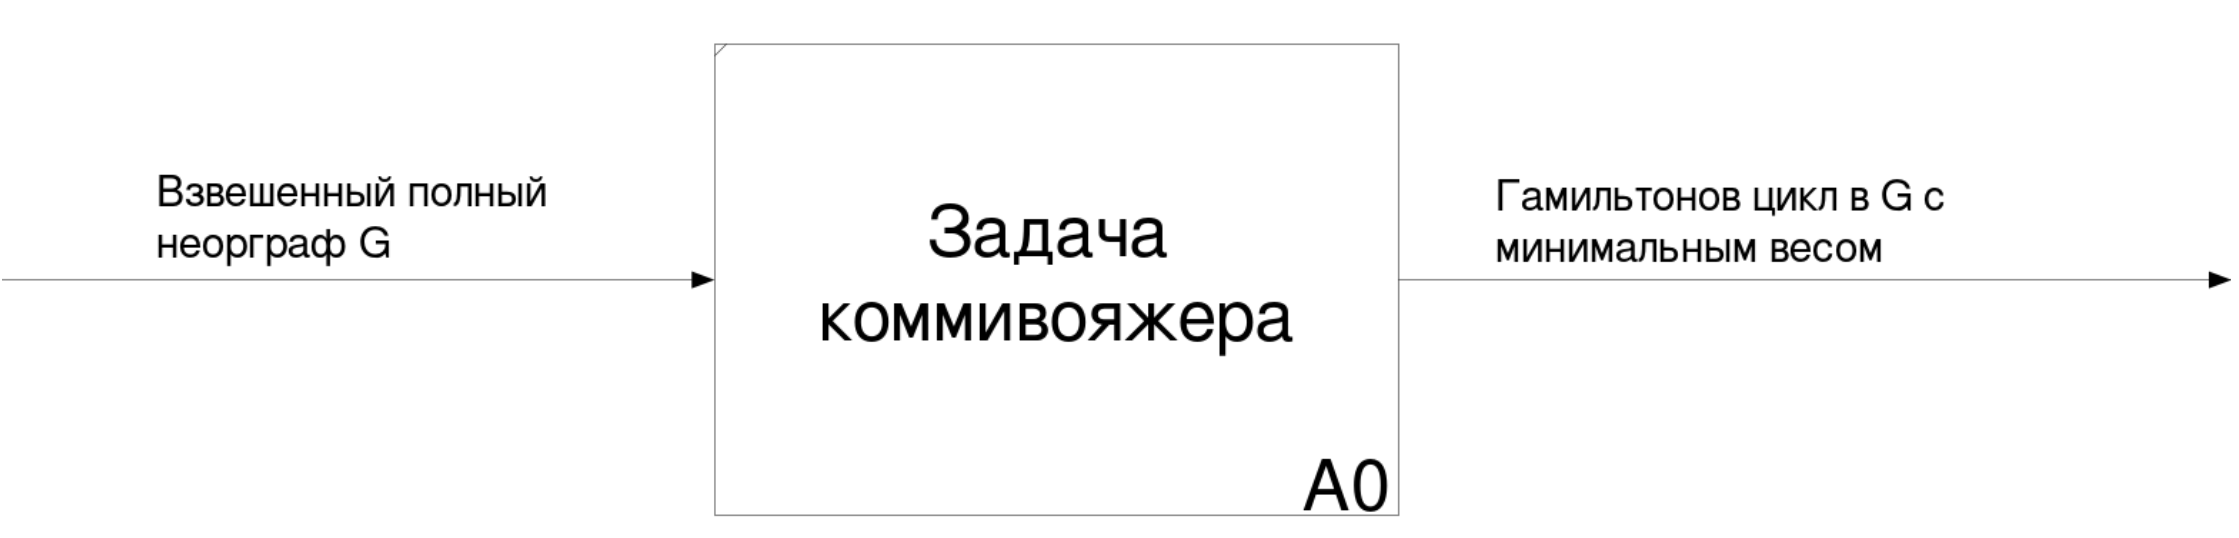
\includegraphics[width=.7\linewidth]{img/idef0.png}
    \caption{Формализованная постановка задачи в нотации IDEF0}
    \label{fig:idef0}
\end{figure}

\section{Методы решения}

В данной работе будут рассмотрены два метода решения задачи коммивояжёра: метод полного перебора и метод муравьиной колонии.

\subsection{Метод полного перебора}

Метод полного перебора подразумевает решение задачи, при котором формируются все возможные гамильтоновы циклы, просчитывается их длина и выбирается тот, у которого эта длина минимальна. Однако с увеличением числа узлов в графе сложность метода существенно возрастает, так как для графа из $n$ узлов существует $\frac{(n-1)!}{2}$ гамильтоновых циклов.~\cite{tsp}

\subsection{Метод муравьиной колонии}

Метод муравьиной колонии -- один из стохастических методов, применяющихся для решения задач комбинаторной оптимизации, в частности для решения задачи коммивояжёра. Метод основан на способе обмена информацией у муравьев, при котором они передают информацию о привлекательности путей с помощью меток (феромонов).~\cite{her}.

\subsubsection{Конструирование путей муравьёв}

На данном этапе каждый из $m$ муравьёв инициализируется с циклом с единственным начальным узлом и на каждом шаге стохастически выбирает узел из тех, которые он не посещал, и добавляет в свой цикл. Выбор узла на очередном этапе цикла производится с вероятностью, вычисляемой по формуле:

\begin{equation}
    p(e^i_j) = \frac{\tau^\alpha_{ij} \cdot f(e^i_j)^\beta}{\sum{\tau^\alpha_{ij} \cdot f(e^i_j)^\beta}},
\end{equation}

где $\tau_{ij}$ - количество феромона на ребре между $i$-м и $j$-м узлами, \newline$f(e^i_j)$ - функция выражающая~«привлекательность»~ребра между $i$-м и $j$-м узлами для муравья.
\subsubsection{Обновление феромонов}

На данном этапе формируются положительные и отрицательные обратные связи. Каждый муравей проходя по своему пути распыляет на нём феромоны, при этом чем длиннее путь, тем меньше распылённое количество феромонов. Распылённое число феромонов для $k$-го муравья рассчитывается по формуле:

\begin{equation}
    \Delta\tau^k_{ij} = \begin{cases} \frac{Q}{L_k}, &\text{если ребро (i, j) есть в цикле муравья}, \\ 0, &\text{иначе}, \end{cases},
\end{equation}

где $L_k$ - длина цикла $k$-го муравья, $Q$ - константа.

Для того, чтобы количество феромона не было решающим фактором после нескольких циклов в модели есть испарение феромона, которое в конце цикла уменьшает концентрацию феромона на каждом ребре.

\subsubsection{Элитные муравьи}

Элитные муравьи -- модификация муравьиного алгоритма. Элитные муравьи на каждой итерации идут по лучшему найденному пути и распыляют по нему феромоны, таким образом увеличиваю привлекательность его частей для других муравьёв. С данной модификацией расчёт феромона на каждой итерации происходит по формуле:

\begin{equation}
    \tau_{ij} = (1-p)\tau_{ij} + \sum_{k=0}^{m}\Delta\tau^k_{ij} + me \cdot \frac{Q}{L_b},
\end{equation}

где $me$ - количество элитных муравьёв, $L_b$ - длина лучшего цикла.

\section{Вывод из аналитической части}

В результате аналитического раздела была рассмотрена формальная постановка задачи коммивояжёра, а также рассмотрены два метода её решения.

\clearpage

\chapter{Конструкторская часть}

\section{Требования к программному обеспечению}

К разрабатываемой программе предъявлен ряд требований:

Входные данные: Взвешенный неориентированный граф, заданный матрицей стоимостей.

Выходные данные: Оптимальный гамильтонов цикл, в случае метода полного перебора, субоптимальный гамильтонов цикл в случае муравьиного алгоритма.

\section{Алгоритм полного перебора}

\subsection{Метод генерации перестановок}

Основной частью алгоритма полного перебора является алгоритм генерации перестановок, так как гамильтонов путь, как и гамильтонов путь, являются перестановками множества узлов графа. Существуют множество методов генерации перестановок~\cite{perms} как рекурсивных, так и итеративных. 
В данной работе будет использоваться нерекурсивный метод Хипа (Heap's method) разработанный в~\cite{perms-methods}.

\subsection{Алгоритм}

На рисунке~\ref{fig:permutations} представлен алгоритм полного перебора для решения задачи коммивояжёра.

\begin{figure}[h]
	\centering
	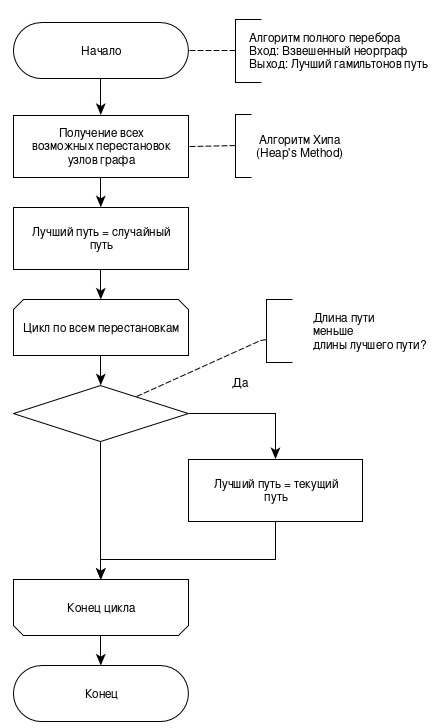
\includegraphics[width=0.6\textwidth]{img/permutations.png}
	\caption{Схема алгоритма полного перебора}
	\label{fig:permutations}
\end{figure}

\clearpage

\section{Муравьиный алгоритм}

На рисунках~\ref{fig:ant1} и~\ref{fig:ant2} представлен алгоритм муравьиного алгоритма для неорграфа с элитными муравьями.

\begin{figure}[H]
	\centering
	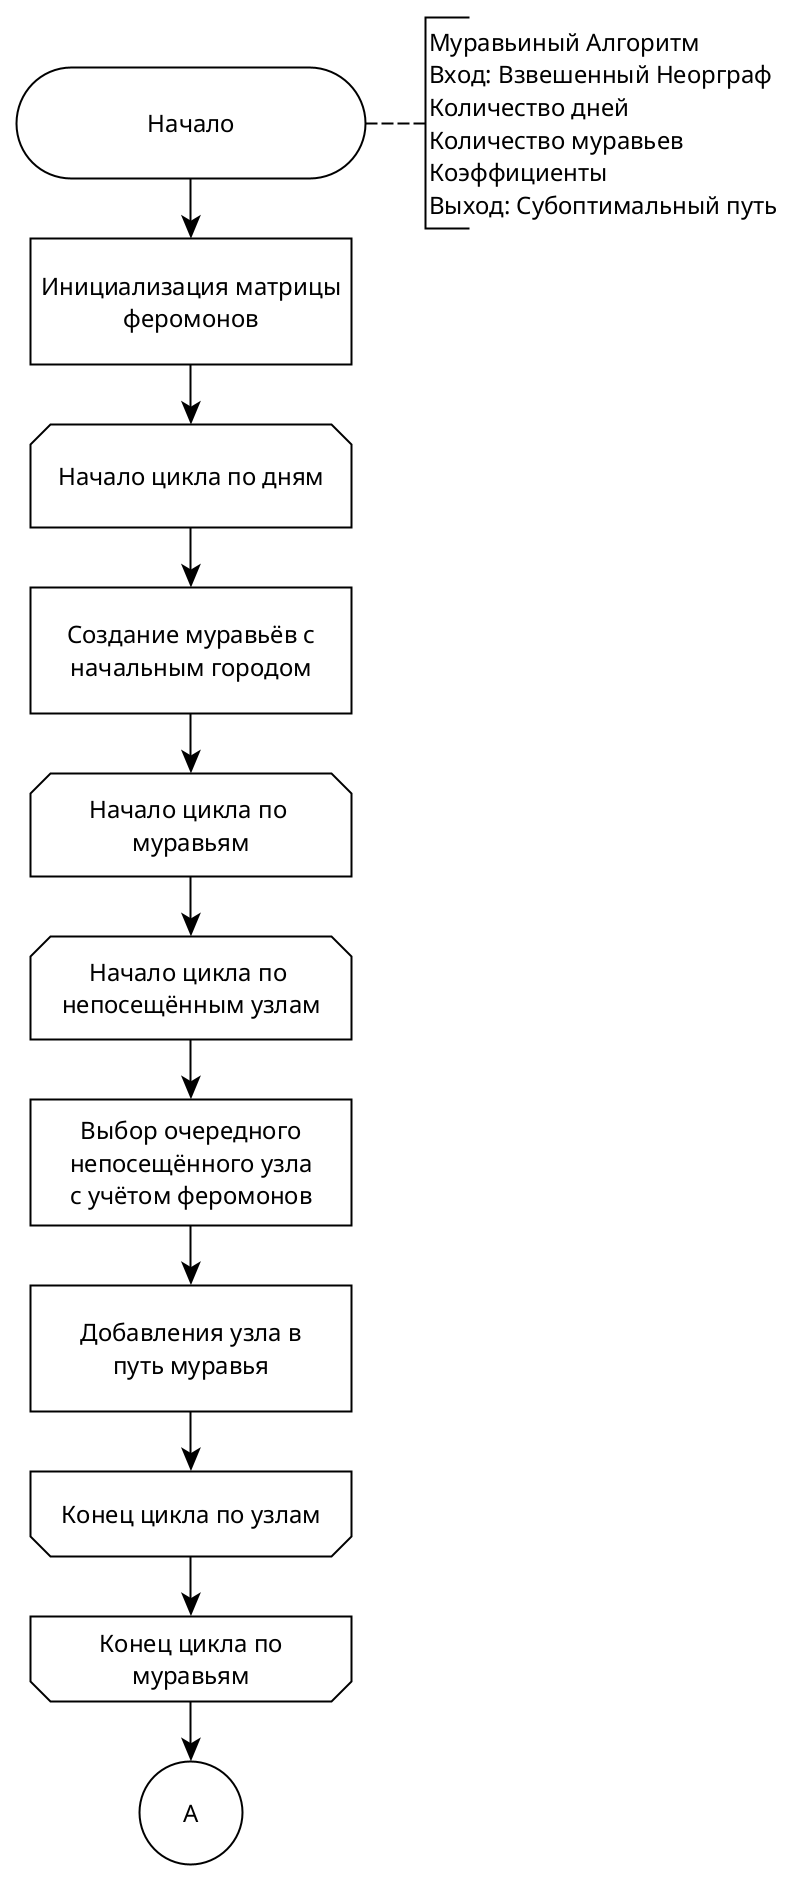
\includegraphics[width=0.5\textwidth]{img/ant1.png}
	\caption{Схема муравьиного алгоритма (начало)}
	\label{fig:ant1}
\end{figure}

\begin{figure}[H]
	\centering
	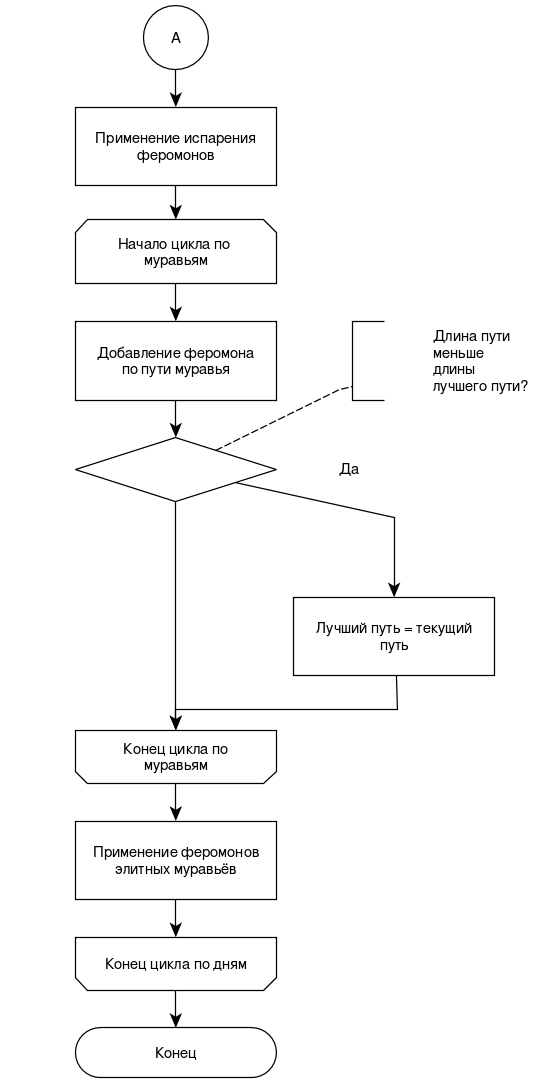
\includegraphics[width=0.45\textwidth]{img/ant2.png}
	\caption{Схема муравьиного алгоритма (конец)}
	\label{fig:ant2}
\end{figure}

\section{Вывод из конструкторской части}

В результате конструкторской части были определены требования к ПО, а также разработаны схемы алгоритмов полного перебора и муравьиного алгоритма.

\clearpage

\chapter{Технологическая часть}

\section{Средства разработки}

В качестве языка программирования был выбран python, так как данный язык обладает достаточными средствами для реализации алгоритмов.

\section{Реализация алгоритмов}

В листинге~\ref{full-search} представлен алгоритма полного перебора.

\begin{lstlisting}[label=full-search,caption={Алгоритм полного перебора},language=python]
def calculate_distance(route, distance_matrix):
    total_distance = 0
    for i in range(len(route) - 1):
        total_distance += distance_matrix[route[i]][route[i + 1]]
    total_distance += distance_matrix[route[-1]][route[0]]
    return total_distance

def find_routes(current_city, visited, route, distance_matrix, all_routes):
    if len(visited) == len(distance_matrix):
        all_routes.append(route[:])
        return

    for next_city in range(len(distance_matrix)):
        if next_city not in visited:
            visited.add(next_city)
            route.append(next_city)
            find_routes(next_city, visited, route, distance_matrix, all_routes)
            route.pop()
            visited.remove(next_city)

def full_search(distance_matrix):
    n = len(distance_matrix)
    all_routes = []
    visited = set()
    
    visited.add(0)
    find_routes(0, visited, [0], distance_matrix, all_routes)

    min_distance = float('inf')
    best_route = None

    for route in all_routes:
        current_distance = calculate_distance(route, distance_matrix)
        if current_distance < min_distance:
            min_distance = current_distance
            best_route = route

    return best_route, min_distance
\end{lstlisting}

В листинге~\ref{ant} представлена реализация муравьиного алгоритма.

\begin{lstlisting}[label=ant,caption={Муравьиный алгоритм},language=python]
import numpy as np
import random

class AntColony:
    def __init__(self, distance_matrix, num_ants, num_iterations, alpha, beta, evaporation_rate, elite_factor, num_elite_ants):
        self.distance_matrix = distance_matrix
        self.num_ants = num_ants
        self.num_iterations = num_iterations
        self.alpha = alpha
        self.beta = beta
        self.evaporation_rate = evaporation_rate
        self.elite_factor = elite_factor
        self.num_elite_ants = num_elite_ants
        self.num_cities = len(distance_matrix)
        self.pheromone_matrix = np.ones((self.num_cities, self.num_cities))

    def run(self):
        best_route = None
        best_distance = float('inf')

        for _ in range(self.num_iterations):
            all_routes = []
            all_distances = []

            for _ in range(self.num_ants):
                route = self.construct_route()
                distance = self.calculate_distance(route)
                all_routes.append(route)
                all_distances.append(distance)

                if distance < best_distance:
                    best_distance = distance
                    best_route = route

            sorted_indices = np.argsort(all_distances)
            elite_routes = [all_routes[i] for i in sorted_indices[:self.num_elite_ants]]
            elite_distances = [all_distances[i] for i in sorted_indices[:self.num_elite_ants]]

            self.update_pheromones(all_routes, all_distances, elite_routes, elite_distances, best_route, best_distance)

        return best_route, best_distance

    def construct_route(self):
        route = []
        visited = set()
        current_city = random.randint(0, self.num_cities - 1)
        route.append(current_city)
        visited.add(current_city)

        for _ in range(self.num_cities - 1):
            next_city = self.select_next_city(current_city, visited)
            route.append(next_city)
            visited.add(next_city)
            current_city = next_city

        return route

    def select_next_city(self, current_city, visited):
        probabilities = []
        total_pheromone = 0.0

        for city in range(self.num_cities):
            if city not in visited:
                pheromone = self.pheromone_matrix[current_city][city] ** self.alpha
                distance = self.distance_matrix[current_city][city]
                probability = pheromone / (distance ** self.beta)
                probabilities.append(probability)
                total_pheromone += probability
            else:
                probabilities.append(0)

        probabilities = [p / total_pheromone for p in probabilities]
        return np.random.choice(range(self.num_cities), p=probabilities)

    def calculate_distance(self, route):
        total_distance = 0
        for i in range(len(route) - 1):
            total_distance += self.distance_matrix[route[i]][route[i + 1]]
        total_distance += self.distance_matrix[route[-1]][route[0]]
        return total_distance

    def update_pheromones(self, all_routes, all_distances, elite_routes, elite_distances, best_route, best_distance):
        self.pheromone_matrix *= (1 - self.evaporation_rate)

        for route, distance in zip(all_routes, all_distances):
            pheromone_deposit = 1.0 / distance
            for i in range(len(route) - 1):
                self.pheromone_matrix[route[i]][route[i + 1]] += pheromone_deposit
            self.pheromone_matrix[route[-1]][route[0]] += pheromone_deposit

        for elite_route, elite_distance in zip(elite_routes, elite_distances):
            elite_pheromone_deposit = self.elite_factor / elite_distance
            for i in range(len(elite_route) - 1):
                self.pheromone_matrix[elite_route[i]]
                [elite_route[i + 1]] += elite_pheromone_deposit
            self.pheromone_matrix[elite_route[-1]][elite_route[0]]
            += elite_pheromone_deposit
\end{lstlisting}

\section{Оценка сложности алгоритмов}

Для алгоритма полного перебора оценка сложности составляет $O(n!*n) = O(n!)$, так как сложность алгоритма генерации перестановок $O(n!)$~\cite{perms-methods}, а сложность поиска цены пути составляет $O(n)$.

У муравьиного алгоритма оценка сложности рассчитывается следующим образом

\begin{equation}
	\label{eq:ant-o}
	O(d * (m * (n^2) + (n^2) + m*n + n)) = O(dmn^2),
\end{equation}
где
\begin{itemize}
	\item d -- количество дней;
	\item m -- число муравьёв;
	\item n -- число узлов.
\end{itemize}

\section{Тестирование}

Тестирование алгоритма полного перебора  возможно провести с проверкой точного значения, однако для муравьиного алгоритма можно проверить лишь то, что результирующий цикл не содержит все узлы, то есть является гамильтоновым циклом.

\subsubsection{Тест 1}

\textbf{Входные данные:}
\[
\begin{bmatrix}
    0 & 10 & 15 & 20 \\
    10 & 0 & 35 & 25 \\
    15 & 35 & 0 & 30 \\
    20 & 25 & 30 & 0 \\
\end{bmatrix}
\]

Ожидаемое значение:

Лучший маршрут: [0, 1, 3, 2]

Минимальное расстояние: 80

Выходные данные полного перебора:

Лучший маршрут: [0, 1, 3, 2]

Минимальное расстояние: 80


Выходные данные муравьиного алгоритма:

Лучший маршрут: [3, 2, 0, 1]

Минимальное расстояние: 80


\subsubsection{Тест 2}

\textbf{Входные данные:}
\[
\begin{bmatrix} 0 & 29 & 20 & 21 & 16 & 31 & 100 & 12 & 4 & 31 \\ 29 & 0 & 15 & 17 & 28 & 40 & 72 & 21 & 29 & 41 \\ 20 & 15 & 0 & 28 & 12 & 25 & 81 & 18 & 24 & 30 \\ 21 & 17 & 28 & 0 & 23 & 39 & 63 & 12 & 18 & 25 \\ 16 & 28 & 12 & 23 & 0 & 30 & 75 & 14 & 21 & 27 \\ 31 & 40 & 25 & 39 & 30 & 0 & 50 & 30 & 35 & 45 \\ 100 & 72 & 81 & 63 & 75 & 50 & 0 & 90 & 100 & 80 \\ 12 & 21 & 18 & 12 & 14 & 30 & 90 & 0 & 10 & 15 \\ 4 & 29 & 24 & 18 & 21 & 35 & 100 & 10 & 0 & 20 \\ 31 & 41 & 30 & 25 & 27 & 45 & 80 & 15 & 20 & 0 \end{bmatrix}
\]


Ожидаемое значение:

Лучший маршрут: [0, 5, 6, 3, 1, 2, 4, 7, 9, 8]

Минимальное расстояние: 241


Выходные данные полного перебора:

Лучший маршрут: [0, 5, 6, 3, 1, 2, 4, 7, 9, 8]  

Минимальное расстояние: 241


Выходные данные муравьиного алгоритма:

Лучший маршрут: [0, 8, 9, 7, 4, 2, 1, 3, 6, 5]  

Минимальное расстояние: 241

\section{Вывод из технологической части}

В ходе технологической части работы были разработаны муравьиный алгоритм и алгоритм полного перебора для задачи коммивояжёра, а также проведена оценка их временной сложности. Все тесты успешно пройдены.

\clearpage

\chapter{Исследовательская часть}

\section{Параметризация}

Параметризация проводится по 3-м параметрам муравьиного алгоритма: $\alpha$ -- коэффициент влияние феромонов на выбор муравья, $p$ -- коэффициент испарения феромонов, дни -- количество дней в муравьином алгоритме.

\subsection{Класс данных}

В качестве класса данных для параметризации используем 3 графа, построенных на морских портах. В качестве весов графа использовались время путешествия между этими портами в днях, взятое из интернет-ресурса route.vesselfinder.com.

Граф 1:
\begin{enumerate}
    \item Rotterdam;
    \item Singapore;
    \item A Coruna;
    \item Abercastle;
    \item Quincy;
    \item Agropoli;
    \item Aigiali Amorgou;
    \item Lulsdorf;
    \item Dortyol;
    \item Heerewaarden.
\end{enumerate}

Граф 2:
\begin{enumerate}
    \item Dresden;
    \item Kostrena;
    \item Marsden Point;
    \item Felixstowe;
    \item Bay Roberts;
    \item Hopewell;
    \item Muasdale;
    \item Carradale;
    \item Orcadas;
    \item Kusadasi.
\end{enumerate}

Граф 3:
\begin{enumerate}
    \item Al Qantarah;
    \item Kwaadmechelen;
    \item Sada;
    \item Hadsund;
    \item Alexandroupolis;
    \item SAXEMARA;
    \item Stokmarknes;
    \item Marsaxlokk;
    \item Miedzyzdroje;
    \item Hoofdplaat.
\end{enumerate}

\subsection{Результаты параметризации}

В результате параметризации оказалось, что самыми лучшими параметрами по заданному классу данных оказались при $\alpha = 0.3$, $p = 0.3$ и количеством дней равным 100. При этом данные параметры дают лучший результат как по средним параметрам, так и по минимальным значениям. Результаты параметризации для данных параметра представлены в таблице~\ref{tbl:d}, а вся таблица параметризации представлена в приложении А.

\begin{table}[H]
    \centering
        \caption{Результаты параметризации муравьиного алгоритма при $\alpha = 0.3$, $p = 0.3$, дни = 100}
    \begin{tabular}{|r|r|r|r|r|r|r|r|r|r|r|r|}
    \hline
    min1 & max1 & mean1 & min2 & max2 & mean2 & min3 & max3 & mean3 \\ \hline
    0 & 0 & 0 & 0 & 0 & 0 & 0 & 0 & 0 \\ \hline
    \end{tabular}
    \label{tbl:d}
\end{table}

\section{Вывод из исследовательской части}

В результате исследовательской части была проведена параметризация по заданному классу данных и выявлены лучшие параметры.

\clearpage

\ssr{ЗАКЛЮЧЕНИЕ}

Цель – рассмотрение методов решения задачи коммивояжёра – была выполнена.
При этом в ходе работы были выполнены следующие задачи:

\begin{itemize}
	\item сформулирована задача коммивояжёра;
	\item рассмотрены методы полного перебора и муравьиной колонии с элитными муравьями;
	\item разработаны рассмотренные алгоритмы решения задачи;
	\item реализованы разработанные алгоритмы;
	\item проведена параметризация для алгоритма на основе метода муравьиной колонии. 
\end{itemize}

В результате работы были проанализированы сложности алгоритмов муравьиной колонии и полного перебора, проведена параметризация муравьиного алгоритма и выявлены лучшие параметры для класса данных, основанных на морских портах, а именно: $\alpha = 0.3$, $p = 0.3$ и количество дней -- 100.

\clearpage

\ssr{ПРИЛОЖЕНИЕ А}